\documentclass[10pt]{article}
\usepackage[margin=0.82in]{geometry}
\usepackage{amsmath,amssymb,booktabs,float,graphicx,microtype}
\usepackage[hidelinks]{hyperref}
\usepackage{xcolor}
\usepackage{tikz}
\usetikzlibrary{arrows.meta,positioning,shapes.geometric}
\newcommand{\RR}{\mathbb{R}}
\newcommand{\E}{\mathbb{E}}
\newcommand{\softmax}{\operatorname{softmax}}
\newcommand{\stopgrad}{\operatorname{stopgrad}}
\title{Olympus: Risk-Monotone Counterfactual Fusion for Governed Multimodal Prediction\\\large Architecture, Controlled Negative Result, and Bounded Engineering Evidence}
\author{Ryan\\Independent Researcher}
\date{October 2026}

\begin{document}
\maketitle

\begin{abstract}
Specialized predictors can expose complementary linguistic, scientific, multimodal,
temporal, and governance signals, yet learned fusion may hide routing collapse and allow
model confidence to weaken external safety information. We specify Olympus, a reference
architecture that projects heterogeneous component states into a common space, emits
leave-one-component-out decisions, derives an intrinsic risk estimate from representation
disagreement, and combines that estimate with a host risk floor through a monotone
noisy-OR. Host-supplied legal-transition masks and a deterministic STOP threshold remain
outside learned authority. We also specify a geometry-conditioned joint-embedding
predictive super-resolution subsystem. We then preregister and execute a controlled
synthetic reliability-shift study with 25 training runs and 75 protected evaluations.
The full mechanism tied parameter-matched uniform fusion on clean accuracy (paired mean
difference $0.000$, 95\% interval $[0.000,0.000]$) and was worse in point estimate on
corrupted selective accuracy ($-0.0469$, $[-0.0953,0.0016]$); the registered hypothesis
is negative. Risk monotonicity and transition legality had zero violations. A separate
24-run study on 36 proprietary instruction records found small loss improvements from
cosine scheduling and validation-best restoration, but exact match was 0\% throughout.
The controlled result does not establish natural-data performance, and the JEPA subsystem
remains unevaluated. The main contribution is therefore a falsifiable architecture,
auditable implementation, and complete negative and blocked-evidence record.
\end{abstract}

\section{Introduction}
Multimodal systems are often evaluated under complete, clean observations even though
missingness, corruption, imbalance, and sample-dependent quality are normal in deployed
settings. Empirical work shows that multimodal Transformers can be sensitive to missing
modalities and that the best fusion strategy is dataset-dependent
\cite{ma2022missing,maheshwari2023m3l}. Mixture-of-experts systems introduce another
failure surface: gates can collapse, experts can be under-trained, and balancing losses
can interfere with the task objective \cite{fedus2021switch,zhou2022expertchoice,wang2024lossfree}.
Uncertainty and selective prediction offer useful diagnostics, but neither ordinary
confidence thresholds nor an architectural score is automatically a calibrated safety
guarantee \cite{geifman2019selectivenet,angelopoulos2022crc,lakshminarayanan2016ensembles}.

We study the following question: can heterogeneous predictors be fused such that marginal
component influence is observable, missing-component sensitivity is directly measurable,
and learned evidence may increase but never decrease a host-declared risk score? The
precise research statement is:

\begin{quote}
Existing fusion approaches struggle to remain auditable and robust when heterogeneous
components are missing, corrupted, or safety-relevant. We propose host-monotone
counterfactual fusion because explicit component interventions and monotone risk
composition predict improved failure detection without allowing learned evidence to
weaken external constraints.
\end{quote}

The candidate novelty is the combined contract, not any ingredient alone. This paper
separates the registered architecture, a controlled synthetic mechanism test, and a
bounded instruction-model case study. The latter tests training infrastructure only.

\section{Related work and novelty boundary}
Joint-embedding predictive architectures learn by predicting target representations from
context rather than reconstructing every pixel. I-JEPA established this principle for
images \cite{assran2023ijepa}; V-JEPA 2 extended it to video, action-conditioned prediction,
and planning \cite{assran2025vjepa2}. The Olympus upscaler borrows the predictive-representation
principle but is not a reproduction of either model.

Sparse MoE work studies conditional computation and routing stability. Switch uses simple
top-1 routing, Expert Choice lets experts select tokens under fixed capacity, and
loss-free balancing adjusts expert-wise routing bias without auxiliary-loss gradients
\cite{fedus2021switch,zhou2022expertchoice,wang2024lossfree}. Olympus presently uses dense
sample-level soft gating, so it cannot claim sparse-compute efficiency.

SelectiveNet jointly learns prediction and rejection and evaluates risk-coverage
tradeoffs \cite{geifman2019selectivenet}. Deep ensembles provide a strong uncertainty and
shift baseline \cite{lakshminarayanan2016ensembles}. Conformal Risk Control controls the
expectation of a monotone loss under its calibration assumptions
\cite{angelopoulos2022crc}. Olympus's monotone noisy-OR is only an algebraic invariant; it
does not provide conformal coverage.

Our search found no exact prior system combining normalized heterogeneous fusion,
first-class leave-one-component-out predictions, disagreement-conditioned risk,
host-monotone risk composition, and host-owned legal transitions. This is a provisional
non-collision result. Independent literature verification remains a release gate.

\section{Problem formulation}
For one independent unit $x$, let $m$ bounded component encoders emit
$h_i\in\RR^{d_i}$. Components may represent text, scientific evidence, workflow traces,
images, temporal state-action histories, or registered extension channels. The system
predicts a task label $y\in\{1,\ldots,C\}$, a next temporal state, a legal research
transition, intrinsic failure risk, and abstention/STOP availability.

The host supplies risk $r_h\in[0,1]$ and a nonempty Boolean legal-transition set $A(x)$.
These are trusted inputs, not model outputs. Training assumes independent source units,
finite tensors, valid labels, and source-disjoint train, calibration, validation, and test
sets. Identifiability of any component's causal contribution is not assumed; leave-one-out
effects are diagnostics unless verified by executed interventions.

The scientific objective is to minimize task, transition, temporal, uncertainty, and
risk losses while controlling routing collapse and component-removal sensitivity. The
primary confirmatory estimand is the paired difference between Olympus and the strongest
matched baseline on a frozen task metric. Secondary estimands cover selective risk,
calibration, corruption robustness, compute, memory, and failure rate.

\section{Model specification}
\subsection{Bounded component families}
Hermes maps byte/token sequences to instruction and tool representations. Prometheus adds
domain adapters and evidence classes. Perseus uses a routed expert bank for workflow
states. Atlas combines token and image-patch representations with retrieval coordinates.
Kronos maps ordered state-action sequences to next-state predictions. Aion maps current
state, effective risk, and host legal transitions to a masked next-stage distribution.
Each reference family is independently executable and shape-checked. Family names describe
interfaces, not frontier capability.

\subsection{Normalized gated fusion}
Each component is projected into a shared width $d$ and normalized:
\begin{align}
z_i &= \operatorname{LayerNorm}(W_i h_i+b_i),\\
g &= \softmax\left(r([z_1;\ldots;z_m])/\tau\right),\\
z &= \operatorname{LayerNorm}\left(\sum_{i=1}^{m} g_i z_i\right),
\end{align}
where $\tau>0$ is fixed before confirmation. The implementation emits $g$, every $z_i$,
and the fused $z$.

\subsection{Counterfactual component output}
For $\epsilon>0$, the leave-one-component-out state is
\begin{equation}
z_{-i}=\operatorname{LayerNorm}\left(
\frac{\sum_j g_jz_j-g_iz_i}{\max(1-g_i,\epsilon)}\right).
\end{equation}
The shared decision head evaluates both $z$ and every $z_{-i}$. A training regularizer may
use
\begin{equation}
L_{\mathrm{cf}}=\E_b\sum_i\stopgrad(g_{bi})
D_{\mathrm{KL}}\left(\stopgrad(p_b)\,\|\,p_{b,-i}\right).
\end{equation}
Because the full prediction is stop-gradient, this term encourages removal robustness; it
does not prove specialization or causal necessity.

\subsection{Disagreement and host-monotone risk}
Let $c$ be the normalized gated centroid. Disagreement and intrinsic risk are
\begin{align}
d &= \frac12\sum_i g_i\left[1-\cos(z_i,c)\right], \quad 0\le d\le1,\\
q &= \sigma(f([z;d])).
\end{align}
With host risk $r_h$, effective risk is
\begin{equation}
r_{\mathrm{eff}}=1-(1-r_h)(1-q).
\end{equation}
Since $r_{\mathrm{eff}}-r_h=q(1-r_h)\ge0$, learned state cannot lower the host risk floor.
This proof is pointwise for bounded inputs. Calibration requires independent labels and a
separate calibration procedure.

\subsection{Governed transitions}
Aion assigns negative infinity to transitions outside $A(x)$. If $r_{\mathrm{eff}}$ reaches
the fixed kill threshold, the selected transition is STOP if STOP is host-allowed;
otherwise execution raises an error. Forced STOP zeroes the externally exposed decision
logits. Raw logits remain available for audit and loss computation but cannot authorize
execution.

\subsection{Objective and complexity}
The joint objective is
\begin{equation}
L=L_{\mathrm{decision}}+\lambda_tL_{\mathrm{transition}}
+\lambda_kL_{\mathrm{temporal}}+\lambda_uL_{\mathrm{hetero}}
+\lambda_rL_{\mathrm{risk}}+\lambda_bD_{\mathrm{KL}}(\bar g\|U)
+\lambda_{\mathrm{cf}}L_{\mathrm{cf}}.
\end{equation}
All weights are finite and nonnegative. The fusion projection costs
$O(\sum_i d_i d)$; dense gating and fusion cost $O(md)$ per example; producing all
counterfactual logits costs $O(mCd)$ in the reference implementation. Component backbone
costs dominate at target scale.

\begin{figure}[H]
\centering
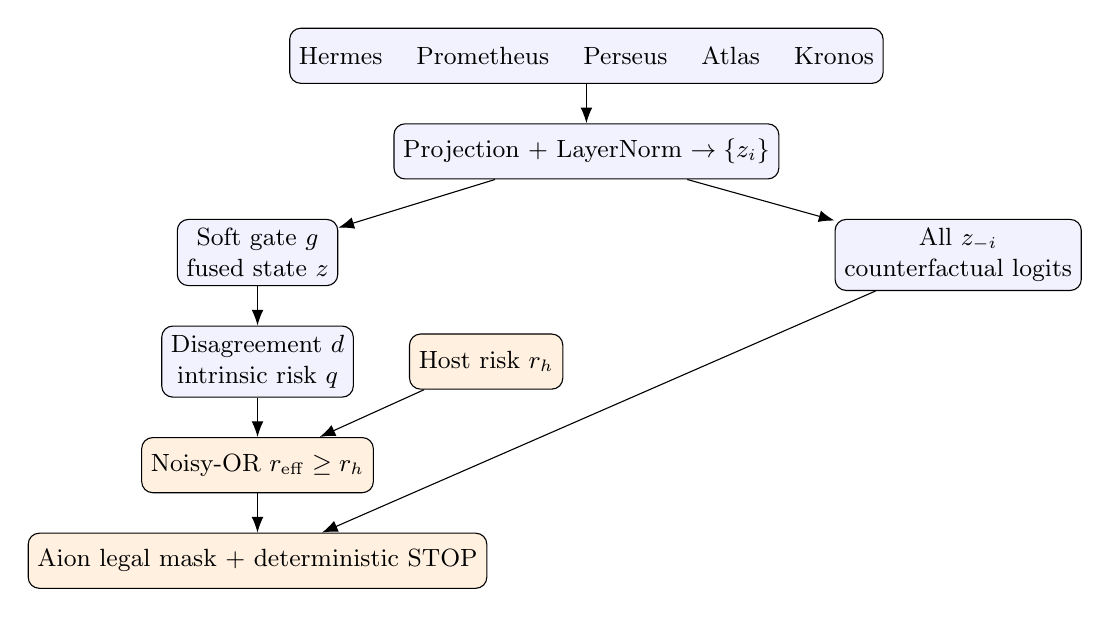
\begin{tikzpicture}[node distance=5mm and 7mm, font=\small,
box/.style={draw, rounded corners, align=center, minimum height=7mm, fill=blue!5},
host/.style={draw, rounded corners, align=center, minimum height=7mm, fill=orange!12},
arr/.style={-{Latex[length=2mm]}}]
\node[box] (families) {Hermes \quad Prometheus \quad Perseus \quad Atlas \quad Kronos};
\node[box, below=of families] (proj) {Projection + LayerNorm $\rightarrow\{z_i\}$};
\node[box, below left=of proj] (gate) {Soft gate $g$\\fused state $z$};
\node[box, below right=of proj] (cf) {All $z_{-i}$\\counterfactual logits};
\node[box, below=of gate] (risk) {Disagreement $d$\\intrinsic risk $q$};
\node[host, right=of risk] (hostrisk) {Host risk $r_h$};
\node[host, below=of risk] (eff) {Noisy-OR $r_{\mathrm{eff}}\ge r_h$};
\node[host, below=of eff] (aion) {Aion legal mask + deterministic STOP};
\draw[arr] (families)--(proj); \draw[arr] (proj)--(gate); \draw[arr] (proj)--(cf);
\draw[arr] (gate)--(risk); \draw[arr] (hostrisk)--(eff); \draw[arr] (risk)--(eff);
\draw[arr] (eff)--(aion); \draw[arr] (cf)--(aion);
\end{tikzpicture}
\caption{Olympus separates learned fusion and intrinsic risk from host-owned risk and
transition authority. Every component-removal output remains observable.}
\label{fig:architecture}
\end{figure}

\section{JEPA super-resolution subsystem}
The upscaler predicts exponential-moving-average target embeddings for high-resolution
patches from masked bicubic context and explicit spatial/temporal coordinates. Its
registered objective combines Charbonnier pixel error, edge error, normalized latent
prediction, latent-gradient geometry, a variance floor, log-magnitude spectrum error,
SSIM, multiscale pyramid consistency, and target-magnitude-weighted phase coherence.
Tiled inference bounds memory. Overlapping predictions use separable squared-sine ramps at
internal boundaries to avoid hard seams without attenuating true outer image edges.
Eight-way dihedral self-ensemble is optional and must be reported as a compute-quality
tradeoff. No reconstruction result is reported because no rights-reviewed source-disjoint
high/low-resolution corpus is available.

\section{Registered evaluation methodology}
The strongest falsifier is a source-disjoint comparison against the best matched single
family, concatenation plus MLP, uniform projected averaging, ordinary softmax gating,
loss-free balancing, and host-risk-only/selective-prediction controls. Parameter-,
activated-FLOP-, information-, and optimizer-budget matching are required. At least five
frozen seeds are used unless a prospective power analysis demands more.

Primary outcomes are paired task quality and selective failure detection. Secondary
outcomes are Brier score, ECE, risk-coverage, unsafe continuation, safe-case STOP,
component-removal delta, OOD shift, corruption, missing modalities, runtime, peak memory,
and energy proxy. Calibration thresholds are chosen only on calibration data. Protected
test outcomes are inspected once. Failed runs, OOM, timeouts, NaNs, and resource rejections
remain in the denominator. Confirmatory primary tests require multiplicity control and
paired confidence intervals.

The repository's aligned dataset contract validates provenance, hashes, source identity,
shape, finiteness, required fields, legal targets, and declared extensions. However, the
rights-reviewed natural aligned corpus does not yet exist. A separately versioned
controlled generator therefore tests the mechanism under known reliability shifts, while
the broader natural-data claim remains blocked.

\section{Controlled synthetic confirmatory study}
\subsection{Protocol and data}
The successor study was frozen before data generation. It created 1,408 source-disjoint
aligned units: 512 train, 128 development, and three protected sets of 256 units each for
clean, double-corruption, and OOD regimes. Each unit contains token, image, temporal
state-action, legal-transition, host-risk, intrinsic-risk, decision, transition, and
next-state fields. The corrupted set removes one modality and independently perturbs a
second. The OOD set additionally increases noise and permutes class-conditional rendering.
Every bundle, manifest, source-ID list, configuration, source file, and checkpoint is
SHA-256 bound.

Five paired seeds trained five parameter-matched variants for 300 steps each: full,
uniform fusion, no counterfactual loss, no disagreement coordinate in the risk head, and
all three mechanisms off. The router is executed even for uniform fusion, but its output
is replaced by exact $1/m$ weights. The primary claim required both a $+0.02$ clean
accuracy improvement and a $+0.03$ corrupted selective-accuracy improvement, with both
paired seed-bootstrap lower bounds above zero. Selective accuracy retains the lowest-risk
half of all examples using raw decision logits. Protected outcomes were opened only after
184 tests, lint, strict typing, and the scientific freeze passed.

\subsection{Confirmatory result}
\begin{table}[H]
\centering
\small
\begin{tabular}{lrrrrr}
\toprule
Variant & Clean acc. & Corrupt acc. & Selective@50 & OOD acc. & Risk Brier\\
\midrule
Full & 1.0000 & 0.8289 & 0.8703 & 0.7227 & 0.7407\\
Uniform & 1.0000 & 0.8664 & 0.9172 & 0.7773 & 0.7397\\
No counterfactual & 1.0000 & 0.8273 & 0.8734 & 0.7211 & 0.7401\\
No disagreement risk & 1.0000 & 0.8289 & 0.8703 & 0.7227 & 0.7483\\
Mechanism off & 1.0000 & 0.8641 & 0.9141 & 0.7758 & 0.7484\\
\bottomrule
\end{tabular}
\caption{Protected means across five independent training seeds. The registered full
mechanism did not outperform exact uniform fusion.}
\label{tab:controlled}
\end{table}

Full-minus-uniform clean accuracy was $0.000$ with paired seed-bootstrap 95\% interval
$[0.000,0.000]$. Corrupted selective accuracy differed by $-0.0469$ with interval
$[-0.0953,0.0016]$. Both practical thresholds failed, so the conjunctive disposition is
\textbf{NEGATIVE}. All 75 protected evaluations had zero host-risk-monotonicity and
transition-legality violations. No secondary ablation contrast survived the registered
Holm adjustment.

\begin{figure}[H]
\centering
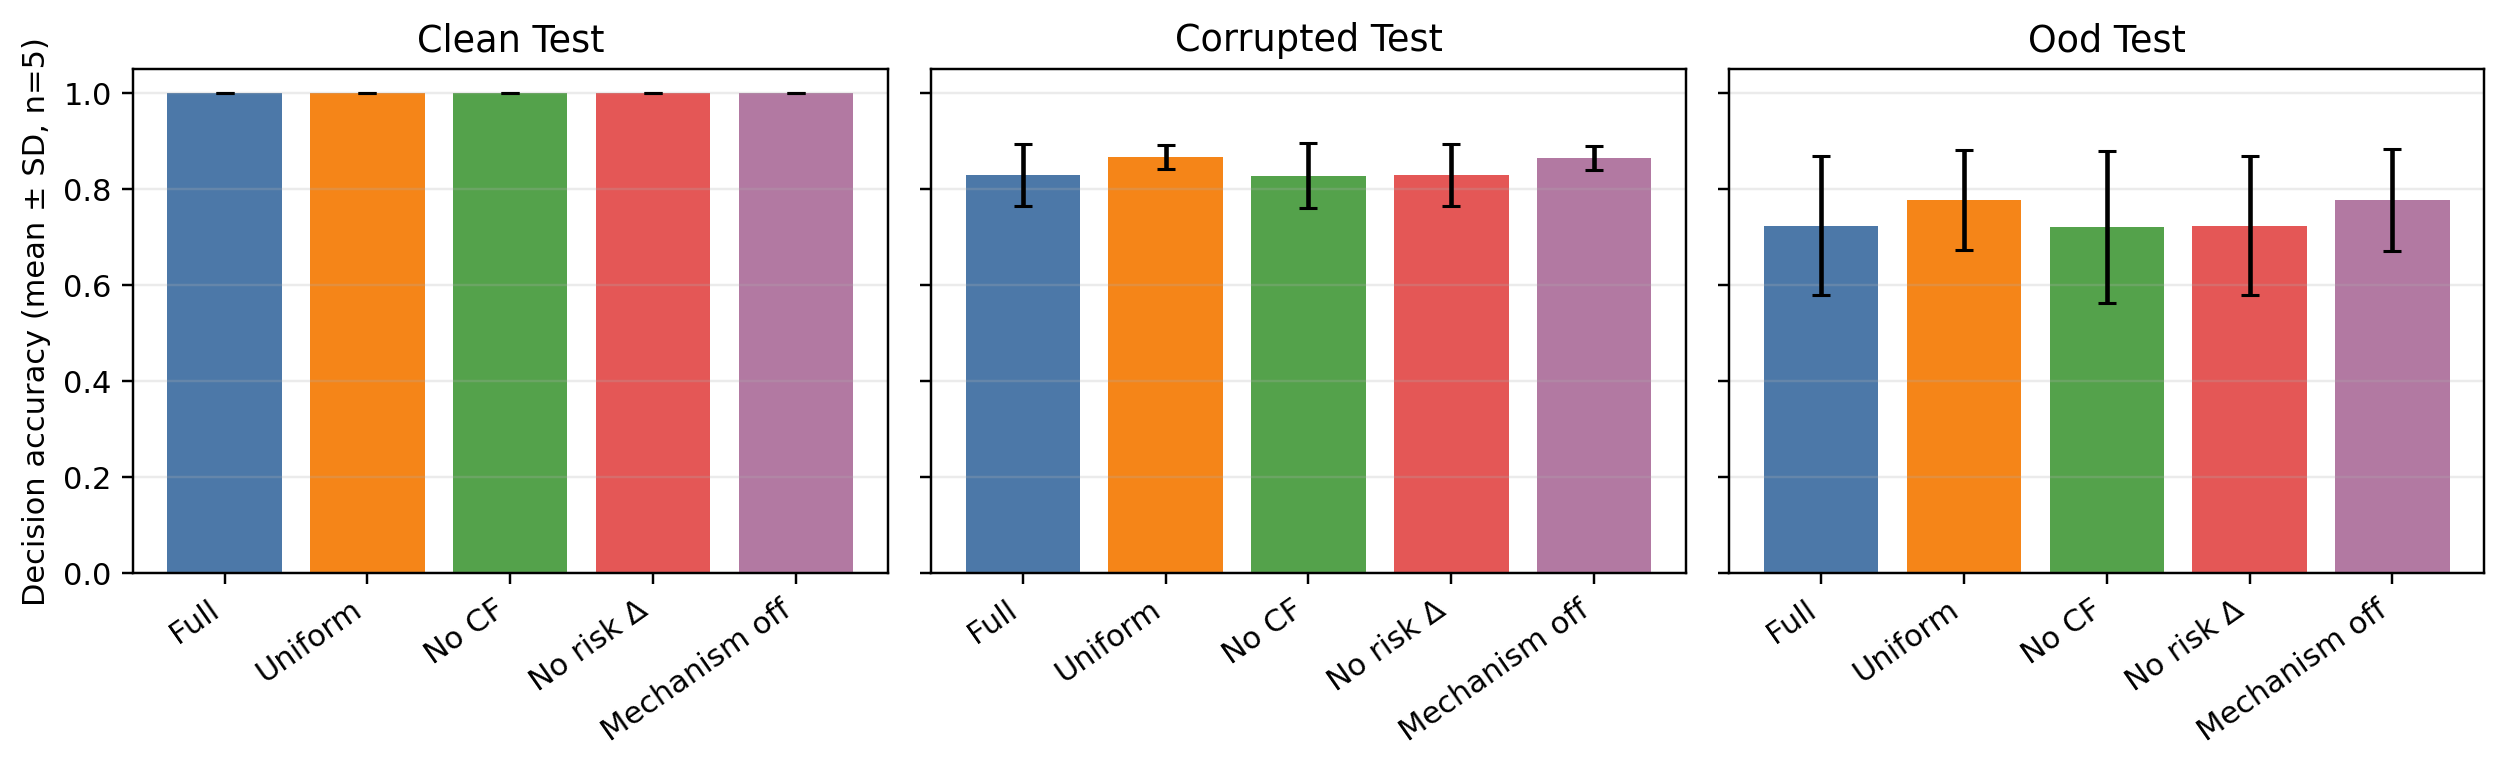
\includegraphics[width=0.98\linewidth]{figures/confirmatory_accuracy.png}
\caption{Protected decision accuracy by regime. Error bars are seed standard deviations,
not confidence intervals. Uniform and mechanism-off controls were more robust under shift.}
\label{fig:confirmatory}
\end{figure}

\begin{figure}[H]
\centering
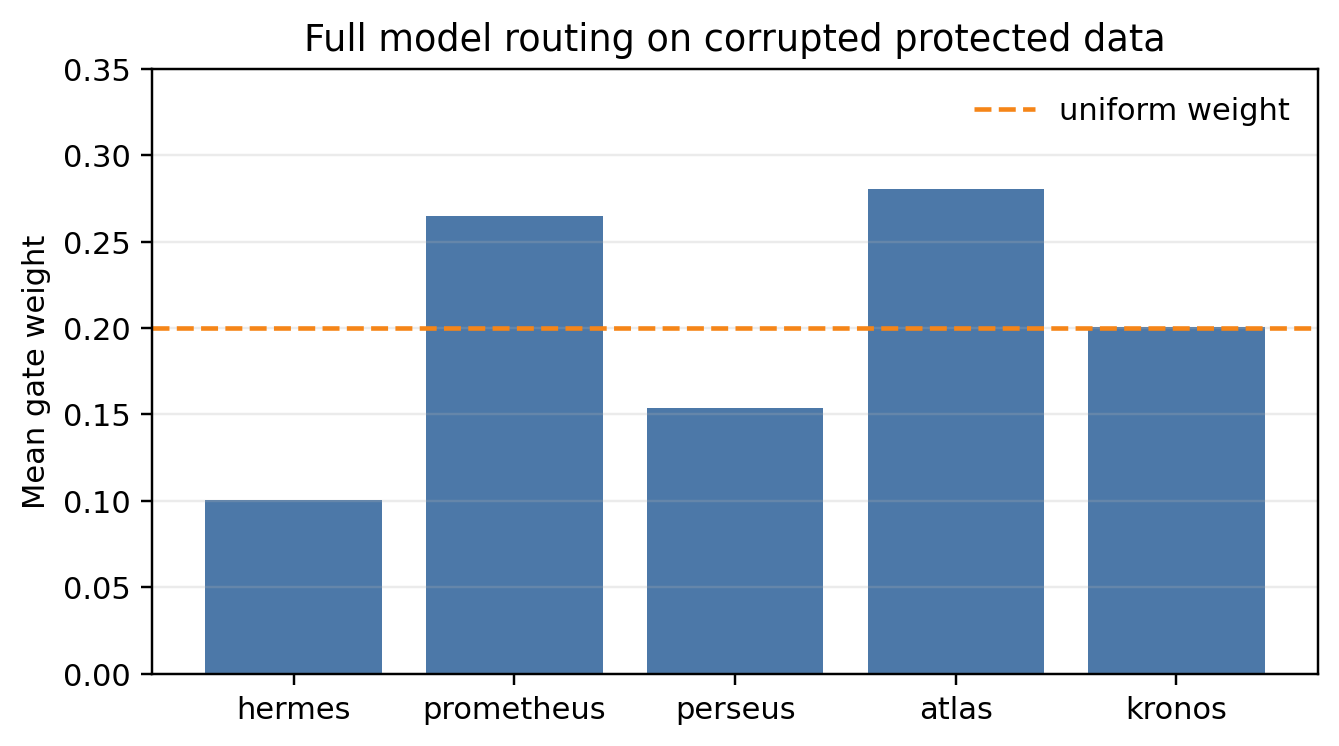
\includegraphics[width=0.68\linewidth]{figures/corrupted_gate_weights.png}
\caption{The full router did not collapse, but moderately over-weighted Atlas and
Prometheus on corrupted data. This source preference was less robust than uniform fusion.}
\label{fig:gates}
\end{figure}

The failure mechanism is consistent with brittle source preference rather than hard gate
collapse: normalized gate entropy was 0.922 and the effective component count was 4.42.
Mean intrinsic risk was only 0.143 on a split with corruption target 1.0, producing a high
0.741 Brier score. Increasing risk supervision or directly supervising reliability after
seeing these outcomes would constitute a new successor hypothesis, not a repair of this
confirmatory result.

\section{Bounded engineering case study}
\subsection{Data and frozen matrix}
The only loaded corpus contains 36 proprietary smoke instruction records, with 12 each in
train, validation, and test. All 12 capability categories occur once per split, and the
manifest reports no exact or contiguous eight-token cross-split duplicate. The test split
had been inspected before this study; all results are development-only.

The frozen matrix contained 24 CPU runs and 900 attempted epochs. Large models had
884,480 parameters; medium models 145,664; small models 35,552. We used byte tokenization,
sequence length 192, batch size 4, gradient accumulation 2, AdamW at $10^{-3}$, weight
decay 0.01, gradient clipping at 1.0, and 30 attempted epochs. Five matched seeds compared
cosine decay, constant rate, and final-epoch versus validation-best state. Three seeds
tested packing and model scale. Learning-rate cosine annealing follows the broad schedule
family introduced by SGDR \cite{loshchilov2016sgdr}, without warm restarts.

\subsection{Results}
\begin{table}[H]
\centering
\small
\begin{tabular}{lrrrr}
\toprule
Variant & Seeds & Parameters & Test loss, mean & Format rate, mean\\
\midrule
Cosine large & 5 & 884,480 & 3.13889 & 0.8333\\
Constant large & 5 & 884,480 & 3.14858 & 0.8333\\
No restore large & 5 & 884,480 & 3.16673 & 0.8333\\
No packing large & 3 & 884,480 & 3.14122 & 0.8333\\
Cosine medium & 3 & 145,664 & 3.44510 & 0.8333\\
Cosine small & 3 & 35,552 & 4.61653 & 0.3889\\
\bottomrule
\end{tabular}
\caption{Exploratory results on an already observed 12-record smoke test. Exact match was
0 in all 24 runs.}
\label{tab:results}
\end{table}

Cosine minus constant test loss averaged $-0.00969$ across five paired seeds with a
deterministic bootstrap 95\% interval $[-0.01607,-0.00564]$. Cosine with validation-best
restoration minus the same schedule at epoch 30 averaged $-0.02784$ with interval
$[-0.03644,-0.02087]$. These intervals quantify seed variation in the frozen matrix; they
do not repair test reuse or establish population-level coverage.

Loss fell with parameter scale, but the comparison was not compute matched. Peak process
RSS was 294,780,928 bytes in the shared process for every recorded evaluation, so it is
not sensitive enough to compare variants. Wall time was contaminated by concurrent host
load and is reported only in raw artifacts.

\begin{figure}[H]
\centering
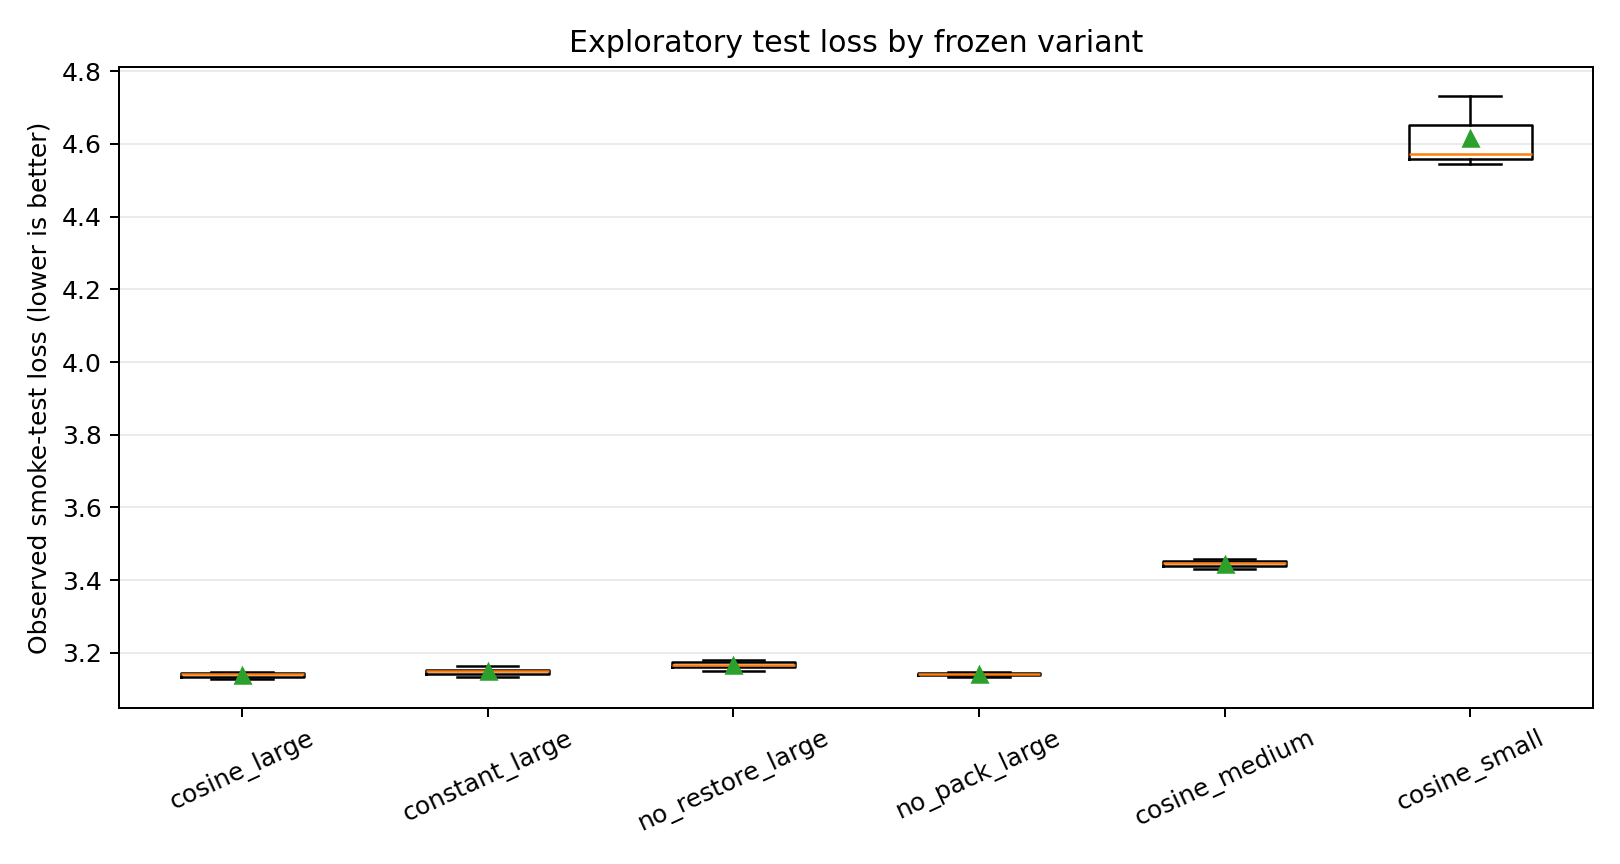
\includegraphics[width=0.82\linewidth]{figures/test_loss_by_variant.png}
\caption{Per-seed exploratory smoke-test loss. The study is not confirmatory.}
\label{fig:loss}
\end{figure}

\begin{figure}[H]
\centering
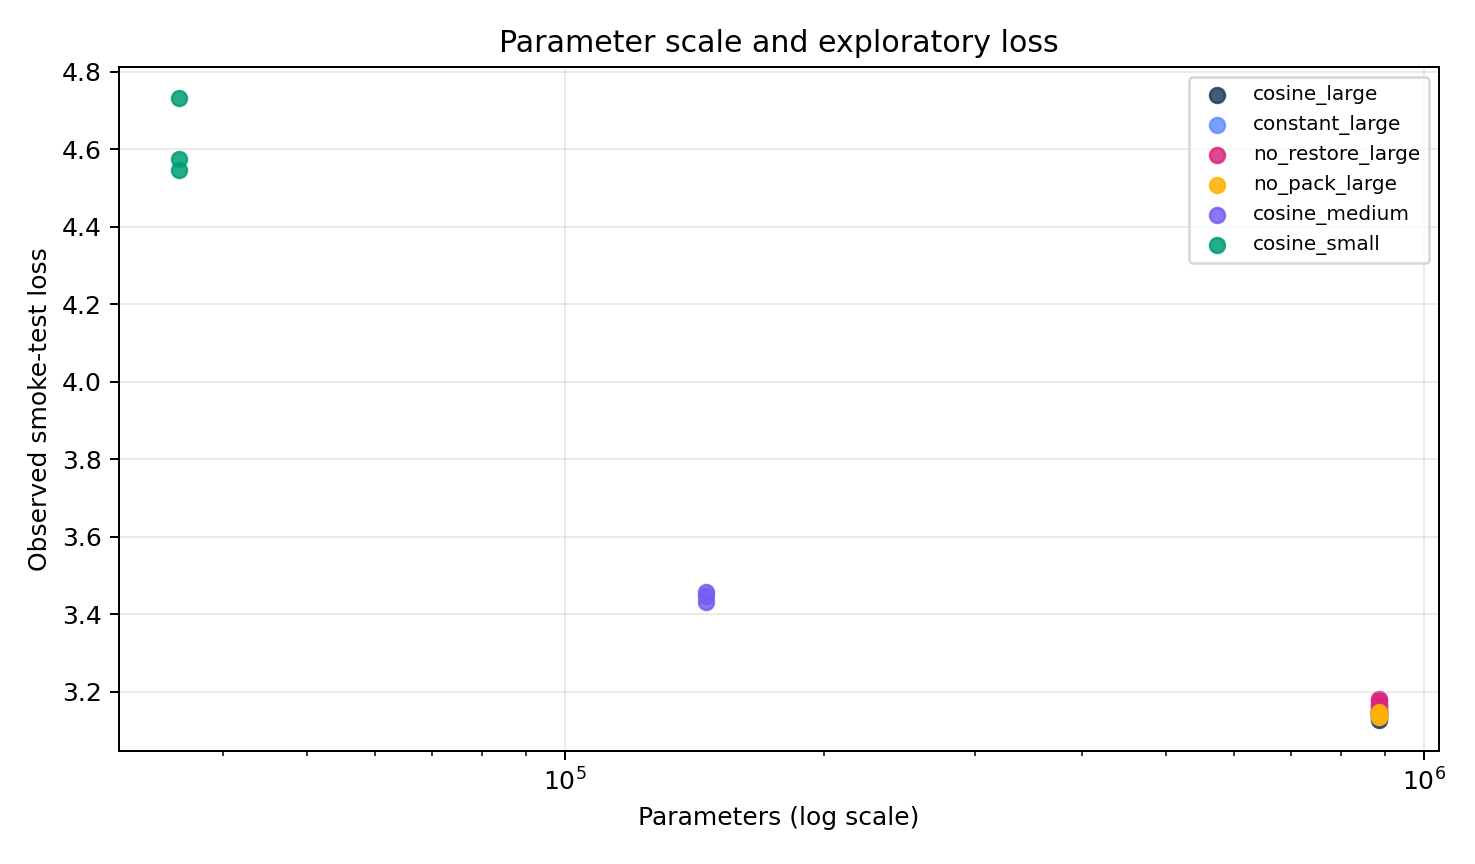
\includegraphics[width=0.78\linewidth]{figures/efficiency_tradeoff.png}
\caption{Parameter scale versus observed test loss. This is a confounded scale ablation,
not a scaling law.}
\label{fig:scale}
\end{figure}

\begin{figure}[H]
\centering
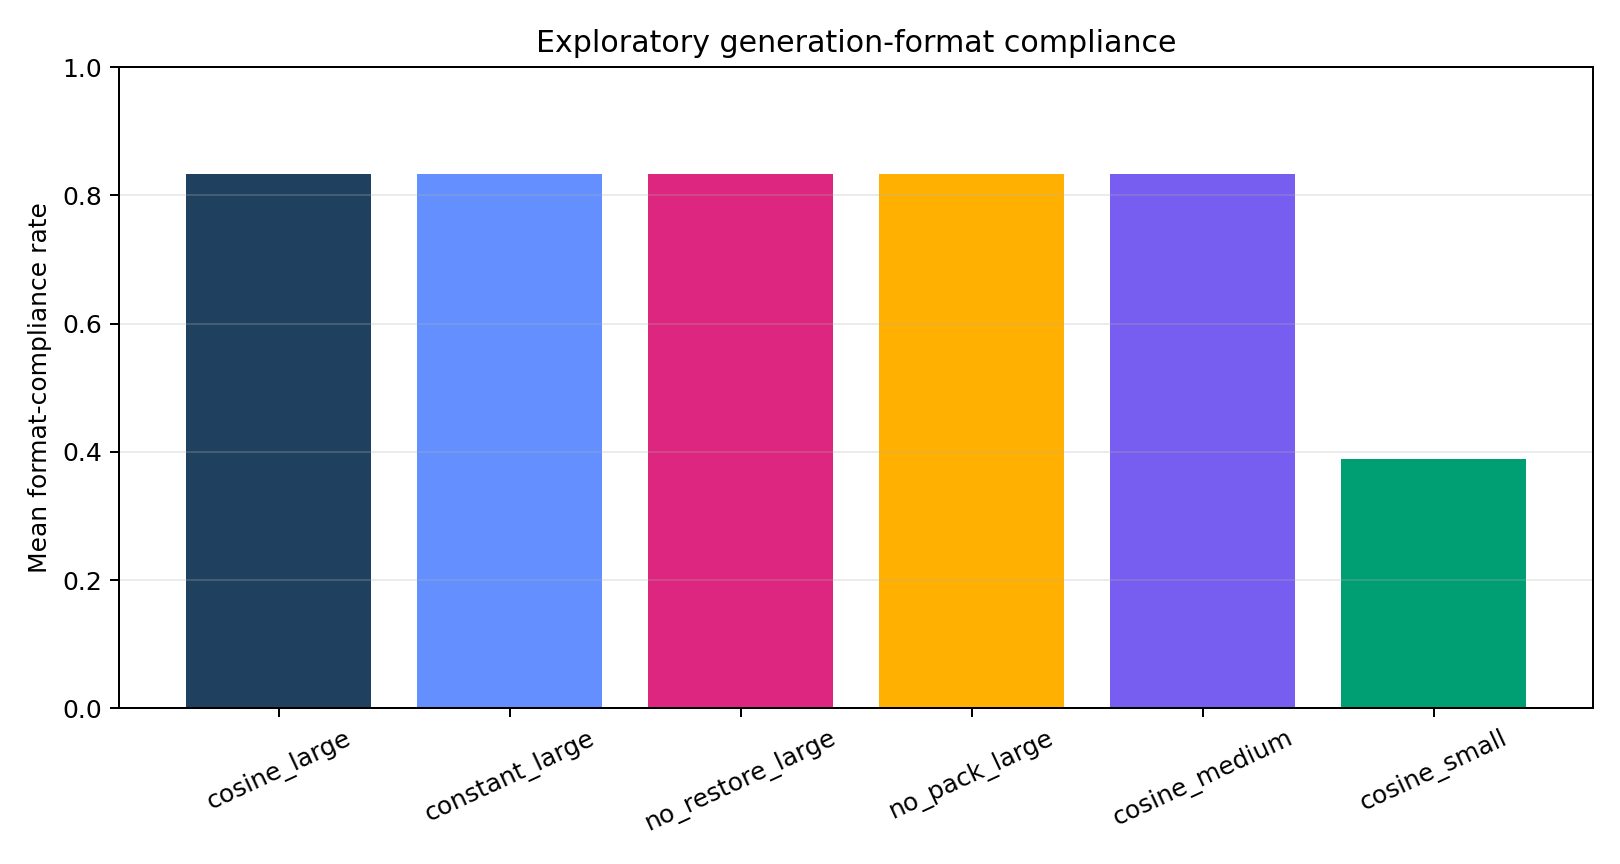
\includegraphics[width=0.82\linewidth]{figures/format_compliance.png}
\caption{Generation-format compliance was stable for medium and large models but highly
variable and lower for the smallest model.}
\label{fig:format}
\end{figure}

\section{Failure and adversarial analysis}
The first matrix attempt was blocked at 91.2\% swap utilization against a frozen 90\%
ceiling. All 24 rejections were retained. The analysis then failed on an empty completed
set; that attempt is invalid, the defect is documented, and the corrected run used a new
artifact root without changing the guard.

The packing intervention was inactive: packing-on and packing-off logs were bit-identical
for shared seeds because examples were already too long to combine under the 192-token
cap. This ablation is non-informative. Most importantly, exact match remained 0\% for all
runs. Lower cross-entropy and acceptable formatting do not imply useful instruction
capability.

Conceptual threats remain substantial: the fusion mechanism may not be novel as a whole;
component influence is not identifiable under substitutable representations; added
parameters, compute, and information can explain gains; joint losses can create gradient
conflict; risk labels can be ambiguous; calibration can fail under shift; and a simpler
linear or uniform fusion may be sufficient. The JEPA objective may also be unnecessarily
complex. The controlled study directly confirmed one of these threats: uniform fusion was
stronger under corruption and OOD. Because three reference families share the same token
channel, the synthetic five-way gate is not five independent modalities; this limits
external interpretation but does not invalidate the registered comparison.

\section{Software verification}
The final repository verification before protected evaluation passed 184 tests with 86.41\%
branch coverage against an 85\% floor. Ruff and strict mypy passed. The frontend test and
production build passed, dependency audits reported no known vulnerabilities in audited
packages, and wheel/sdist construction plus metadata checks passed. Tests cover shapes,
gradients, finite losses, forbidden transitions, monotone risk, STOP behavior, extension
channels, content-addressed data, immutable checkpoints, JEPA tiling, and end-to-end
reference execution. These are software claims, not scientific validation.

\section{Limitations and disposition}
No rights-reviewed natural aligned multimodal/temporal/governance corpus exists in the
repository. The controlled generator provides causal clarity but not natural-image,
natural-language, organizational-workflow, or deployment validity. The smoke test is tiny
and contaminated for fresh confirmation. The JEPA subsystem still has no source-disjoint
reconstruction evaluation. The literature search was broad but not independently
reproduced. Reference-scale behavior may not survive scaling.

Accordingly, the controlled successor result is \textbf{NEGATIVE}: the registered learned
fusion package did not beat uniform fusion under its tested reliability shifts. The broad
natural-data Olympus question remains \textbf{INCONCLUSIVE / NOT EVALUATED}. The bounded
engineering case study is \textbf{MIXED}: two training safeguards improved an already
observed loss measure, scale correlated with lower loss, packing was non-informative, and
exact-match capability remained zero. Promotion and deployment are not authorized.

\section{Reproducibility and release statement}
The predecessor and successor canonical states record their questions, budgets, protected
boundaries, data hashes, failures, decisions, and histories. The successor scientific
freeze binds 25 configurations and checkpoints before 75 protected evaluations. Every
run retains raw metrics and invariant counts; aggregate JSON, CSV, figures, invalid
orchestration receipts, and render receipts are preserved. Reproduction commands are
provided with the source. This manuscript and package are arXiv-ready as a registered
architecture with an honest controlled negative result, not as a positive capability
paper. External submission was not performed.

\section{Conclusion}
Olympus makes a narrow architectural promise: learned evidence cannot lower host risk,
legal transitions remain host-owned, and every component-removal decision is auditable.
The implementation and controlled pipeline work end to end, and all tested invariants
held. The stronger empirical claim failed: learned gates and the registered regularizers
did not improve controlled reliability-shift robustness over uniform fusion. The result
suggests that routing needs explicit reliability identification rather than merely a
learned source preference. The broader natural-data and JEPA questions remain open.

\appendix
\section{Future natural-data confirmatory matrix}
A future, separately versioned study must include best-family, concatenation, uniform, ordinary-gate,
loss-free balance, host-only risk, entropy, SelectiveNet, deep-ensemble, and every
leave-one-family-out baseline. It must test modality deletion, corruption, source and
temporal shift, risk-label perturbation, gate temperature, objective weights, dataset and
model scale, frozen versus joint backbones, and JEPA loss terms. All configurations,
practical effect thresholds, exclusions, and stopping rules are frozen before protected
outcomes.

\section{Artifact inventory}
Primary artifacts include both canonical JSON states, both protocols, the literature
review, successor result audit and evidence map, reproduction instructions, immutable
failure attempts, 25 controlled checkpoints, 75 protected records, locked summary,
aggregate table, figures, corrected 24-run engineering root, source, bibliography, PDF,
and arXiv package. Proprietary dataset records are excluded unless distribution rights
are established. The staged EditCLEVR metadata is CC BY 4.0 but its image payload is not
bundled.

\bibliographystyle{plain}
\bibliography{references}
\end{document}
